In computational linear algebra, we would spend a lot of time in matrix equations or expressions like $Ax = b$. However, for large matrices  $A$, it is always difficult and inefficient to find the value of $x$, if we try finding the inverse of $A$ directly. So what we want to do is to "transform" our $A$ into smaller building blocks with specific properties, and use their properties of them to make the equation easier to solve. 

\medskip
\noindent The transformations, should preserve the correctness in matrix calculations (be sufficiently free from truncation errors, as said in the \href{https://comp-lin-alg.github.io/L2_QR_factorisation.html#what-is-the-qr-factorisation}{\textbf{Introduction}} of Chapter 2), and be efficient enough to perform. Here, let us talk about the very first transformation, the \textbf{QR Factorisation}. 
\medskip

\noindent You might have seen this in your year 2 \href{https://github.com/Imperial-MATH50003/MATH50003NumericalAnalysis}{Numerical Analysis} Course, and make some progress in implementation using Julia or Python. We would do some recap and dig further into algorithm stability, and/or time complexities with different ways of implementations.
\newpage
\section{QR Factorisation Concept}%
\begin{definition}[Complete QR Factorisation]
  The \textbf{Complete QR Factorisation} is defined as the processing of decomposing an arbitrary matrix $A \in \mathbb{C}^{m \times  n}$ to the form
  \[
    A = QR \text{ where } Q \text{ unitary } \in \mathbb{C}^{m \times m}, R  \text{ upper triangular } \in \mathbb{C}^{m \times n}
  .\]
\end{definition}
Without loss of generality we consider $m > n$, and have:
\[
\underset{\begin{array}{c}\\ A \end{array}}%
{
\begin{pmatrix}
  a_{11} & a_{12} & \ldots & a_{1n} \\
  a_{21} & a_{22} & \ldots & a_{2n} \\
  \vdots & \vdots & \ddots & \vdots \\
  a_{m1} & a_{m2} & \ldots & a_{mn}
\end{pmatrix}
}
=
\underset{\begin{array}{c}\\ Q \end{array}}%
{
\begin{pmatrix}
  q_{11} & \ldots & q_{1n} & \ldots & q_{1m} \\
  q_{21} & \ldots & q_{2n} & \ldots & q_{2m}\\
  \vdots & \ddots & \vdots & \ddots & \vdots\\
  q_{m1} & \ldots & q_{mn} & \ldots & q_{mm}
\end{pmatrix}
}
\begin{spmatrix}{R}
  r_{11} & r_{12} & \ldots & r_{1n} \\
  0 & r_{22} & \ldots & r_{2n} \\
  0 & 0 & \ldots & r_{3n} \\
  \vdots & \vdots & \ddots & \vdots \\
  0 & 0 & \ldots & r_{nn} \\
  \vdots & \vdots & \ddots & \vdots \\
  0 & 0 & \ldots & 0
\end{spmatrix}
\]
Note that, the term $q_{ik}r_{kj}$ would always give out 0 when $k > n$ and make no contribution to the value of  $a_{ij}$. Therefore, we could only consider the first $n$ columns of $Q$ and the first $n$ rows of $R$ as the result of factorisation.

\begin{definition}[Reduced QR Factorisation]
  The \textbf{Reduced QR Factorisation} is defined as the processing of decomposing an arbitrary matrix $A \in \mathbb{C}^{m \times  n}$ to the form
  \[
    A = \hat{Q}\hat{R} \text{ where } \hat{Q} \text{ unitary } \in \mathbb{C}^{m \times n}, \hat{R}  \text{ upper triangular } \in \mathbb{C}^{n \times n}
  .\]
  where \(\hat{Q}\), \(\hat{R}\) are sub-matrices of the  complete factorisation results \(Q\), \(R\).
\end{definition}
We are mainly talking about the \textbf{reduced} case of QR factorisation in this chapter, but do think about the complete case when doing exercises.

\subsection*{Exercise 2.3: Find an orthonormal basis of the orthogonal complement of a subspace}
\addcontentsline{toc}{subsection}{Exercise 2.3: Find an orthonormal basis of the orthogonal complement of a subspace}
\subsubsection*{Problem Description}%
\label{ssub:problem_description}

Given a set of vectors $ \{v_1, v_2, \ldots, v_n\}$ spans subspace $U \subset \mathbb{C}^{m}$, we need to find an orthonormal basis of its orthogonal complement $U^{\bot}$, defined as:
\[
U^{\bot} = \{x \in \mathbb{C}^{m}: \forall u \in U, x^{*}u = 0\} 
.\] 
Implement this as a function \href{https://comp-lin-alg.github.io/cla_utils.html#cla_utils.exercises2.orthog_space}{\texttt{exercises2.orthog\_space()}}. \medskip

\subsubsection*{Hints}
\begin{enumerate}
  \item Consider the condition \(\forall u \in U, x^{*}u = 0\), can we consider the elements in a smaller \textbf{subset of \(U\)} rather than all elements in \(U\) to simplify the satisfying criteria? If so, what is the subset?
  \item You might find the matrix \(Q\), \(R\) from complete factorisation useful for answering the question above.    
  \item Consider the matrix \(Q\) obtained from the \textbf{complete QR factorisation}, what is the relationship between any two columns of \(Q\)?  
  \item You might want to use the numpy-based QR factorisation routine \texttt{numpy.linalg.qr()}.
\end{enumerate}
If you have the answer to the questions above, you have already got the key to solving this problem. Pause here for a moment to think about how to obtain the orthonormal basis of \(U^{\bot}\). Feel free to read my explanation on the next page if you get confused. \medskip

\noindent \textbf{Remember to check your implementation passes the provided test cases.}
\newpage

\subsubsection*{Spoil Alert \ldots There is a way you could figure out the problem:}%
\begin{itemize}
\item The first thing we need to figure out is, we are finding the vectors that are \textbf{orthogonal to the basis} of \(U\). This could be obtained by the first \(n\) columns in matrix \(Q\) from the complete QR of \(U\).
\item Then we consider the matrix \(Q\). Given that $Q$ is unitary, we would see all column vectors are orthogonal to each other by expanding
  \[
    [Q^*Q]_{ij} = q_i^*q_j = \delta_{ij} = \left\{
      \begin{array}{l}
      0 \text{ when $i \neq j$} \\
      1 \text{ when $i = j$}
      \end{array}
    \right.
  .\] 
  \item We need to find the vectors that are orthogonal to the first \(n\)  column vectors in $Q$, i.e. columns of \(\hat{Q}\). And we could see the remaining $m - n$ columns in  $Q$ are indeed orthogonal to any vector in the first n columns, by the mutual orthogonality mentioned above. 
  \item Therefore, what we need to do is just to find the \textbf{last} $m - n$ \textbf{columns} from $Q$, which should should be the basis of the orthogonal complementary $U^{\bot}$. \checked
\end{itemize}

\newpage
\section{QR Factorisation by Classical Gram-Schmidt}%
We have already seen the concept of QR factorisation, and one of the applications through the previous exercise. Then we are going to explore what exactly happens in this factorisation, via algorithms. The first implementation we would discuss would be the \textbf{classical Gram-Schmidt algorithm}. The algorithm itself is straightforward:
\begin{algorithm}
  \caption{Classical Gram-Schmidt Algorithm}
  \begin{algorithmic}[1]
  \Procedure{GS\_classical}{A}
    \State initialise \(Q, R\)  as empty matrices
    \For{ \(j = 1\) to \(n\)}
      \State \(v_j = a_j\)
      \For{ \(i = 1\) to \(j - 1\)}
        \State \(r_{ij} = q_i^{*}a_j\)
        \State \(v_j = v_j - r_{ij}q_i\)
        \Comment{Remove components of existing \(q_i\) from \(v_j\)}
      \EndFor
      \State \(r_{jj} = \|v_j\|\)  
      \State \(q_j = \frac{v_j}{\|v_j\|}\)
      \Comment{Finish constructing a new basis vector \(q_j\)}
    \EndFor
    \State \Return \(Q, R\)
  \EndProcedure
  \end{algorithmic}
\end{algorithm}

\noindent However, the algorithm might look no sense at all since we haven't discussed the maths behind it so far. Here we look backwards to see how vectors $ \{a_i\} $ factorised to orthonormal vectors $ \{q_i\} $. \medskip

\noindent Just expand $A = QR$ by arithmetic:

 \[
   A = QR \implies \begin{pmatrix} a_1 & a_2 & \ldots & a_n \end{pmatrix} = 
   \begin{pmatrix} 
     q_1 & q_2 & \ldots & q_n 
  \end{pmatrix} 
   \begin{pmatrix} 
     r_{11} & r_{12} & \ldots & r_{1n} \\ 
     0 & r_{22} & \ldots & r_{2n} \\
     \vdots & \vdots & \ddots & \vdots \\
     0 & 0 & \ldots & r_{nn}
   \end{pmatrix}  
.\] 
So we could see the value of any column vector $a_j$ via column-space interpretation and get:
\[
  a_j = 
   \begin{pmatrix} 
     q_1 & q_2 & \ldots & q_j & \ldots & q_n 
  \end{pmatrix} 
  \begin{pmatrix} r_{1j}\\ r_{2j} \\ \vdots\\ r_{jj} \\ 0 \\ \vdots \\ 0 \end{pmatrix}
\] 
\[
  = r_{1j} q_1 + r_{2j}q_2 + r_{3j}q_3 + \ldots + r_{jj}q_j + 0 \cdot q_{j + 1} + \ldots + 0
  = \sum_{i=1}^{j} r_{ij}q_i
.\] 
Starting with $a_1$, we could see that:
 \[
a_1 = r_{11} q_1
.\] 
and in this expression we could observe $q_1$ is the unit vector parallel to $a_1$, so $r_{11}$ and $q_1$ should have the value
\[
r_{11} = \|a_1\| \text{ and } q_1 = \frac{a_1}{\|a_1\|} = \frac{a_1}{r_{11}}
.\]
Then consider $a_2$ from the summation expression above:
 \[
a_2 = r_{12}q_1 + r_{22}q_2
.\]
But we don't know how to get the value of $r_{12}$ yet. Since we know $a_2 = r_{22}q_2 + r_{12}q_1$, and here is the trick to find \(r_{12}\) by using \(q_1\)  :
\[
  q_1^* a_2 = r_{22}(q_1^{*}q_2) + r_{12}(q_1^{*}q_1) = r_{22} \cdot 0 + r_{12} \cdot 1 = r_{12}
.\]
and to get the value of $q_2$ and $r_{22}$, we remove the component of $q_1$ from $a_2$ and we could get:
\[
    v_2 = a_2 - r_{12}q_1 = r_{22}q_2 \implies 
    \left\{
      \begin{array}{l}
      r_{22} = \|v_2\| \\
      q_2 = \frac{v_2}{\|v_2\|} = \frac{v_2}{r_{22}}
      \end{array}
    \right.
.\]
Then we should have an orthonormal set $ \{q_1, q_2\} $, and we could compute corresponding $q_3$ and scale factor $r_{i3}$s in a similar approach. \medskip

\noindent As we repeat these steps iteratively, we could compute the value of $q_4, q_5, \ldots$ until $q_n$, and also the coefficients \(r_{ij}\). And more generally, given matrix \(A \in \mathbb{C}^{m \times n}\), we could compute the entries of \(Q \in \mathbb{C}^{m \times  n}, R \in \mathbb{C}^{n \times  n}\) with the following formula:
\[
  q_j = \frac{v_{j}}{\|v_{j}\|}
\]
\[
  r_{ij} = \left\{
    \begin{array}{ll}
    q_{i}^{*}a_{j} & i < j\\
    \|v_{j}\| & i = j\\
    0 & \text{otherwise}
    \end{array}
  \right.
  \]
  where
  \[
    v_{j} = \left\{
      \begin{array}{ll}
        a_{j} & i = 1\\
        a_{j} - \sum_{k=1}^{j - 1} r_{kj}q_{k} = a_{j} - \sum_{k=1}^{j - 1} (q_{k}q_{k}^{*})a_{j} & \text{otherwise}
      \end{array}
      \right.
      \]
      Now the algorithm above should be easy for you to understand. \checked

\noindent \textbf{Important! Please make sure you understand the gist behind the contents below.}  The expressions of \(r_{ij}\) and \(v_j\) look messy and complex to implement in python. Here we have a concise and elegant way to find the values of \(r_{ij}\) and \(v_j\) via matrix products.
\[
  r_j = \begin{pmatrix} r_j^{(j - 1)} \\ r_{jj} \\ 0 \\ \vdots \\ 0\end{pmatrix} = \begin{pmatrix} Q_{(j - 1)}^{*}a_j \\ \|v_j\| \\ 0 \\ \vdots \\ 0\end{pmatrix}
  \]
  where \(Q_{j - 1} = \begin{pmatrix} 
  q_1 & \dots & q_{j - 1} 
\end{pmatrix} \) and \(r_j^{(j - 1)} = \begin{pmatrix} 
  r_{1j} & \dots & r_{(j-1)j}
\end{pmatrix} \), with   
\[
  v_j = a_j - Q_{j - 1}r_j^{(j - 1)} = a_j - Q_{j - 1}(Q_{j - 1}^{*}a_j) = (I - Q_{j - 1}Q_{j - 1}^{*})a_j
\]
Note that the \(^{*}\) here \textbf{refers to the adjoint of a matrix}, not the scalar multiplication!
\textbf{Do pause here for a while to make sure you could show the expressions above by yourself.} \medskip

\noindent 
You can see we are now eliminating the index \(i\) in every expression by replacing the summation with matrix products. This is essential since you can get rid of one for-loop with variable \(i\)  in the algorithm above, and use NumPy-based matrix multiplication. \smallskip

\noindent Since we've seen the fact that using matmul in NumPy is more efficient than using for loops, you should pay more attention to using more "vectorized operations" like matmul, and \textbf{reduce for loops as much as possible. }

\noindent Here is the optimised version of the classical Gram-Schmidt algorithm, \textbf{which is not mentioned by the lecturer} but you would \textbf{lose marks if not optimised.}
\begin{algorithm}
  \caption{Classical Gram-Schmidt Algorithm, optimised}
  \begin{algorithmic}[1]
  \Procedure{GS\_classical\_optimised}{A}
    \State initialise \(Q, R\)  as empty matrices
    \For{ \(j = 1\) to \(n\)}
      \State \(r_j^{(j - 1)} = Q_{(j - 1)}^{*}a_j\)
      \State \(v_j = a_j - Q_{j - 1}r_j^{(j - 1)}\)
      \State \(r_{jj} = \|v_j\|\)
      \State \(q_j = \frac{v_j}{\|r_{jj}\|}\)    
    \EndFor
    \State \Return \(Q, R\) 
  \EndProcedure
  \end{algorithmic}
\end{algorithm}

\newpage
\noindent To let you have a more direct sense of classical Gram-Schmidt, \autoref{cgs} would demonstrate the flow of the classical Gram-Schmidt Algorithm. 
\begin{figure}[htp]
  \centering
  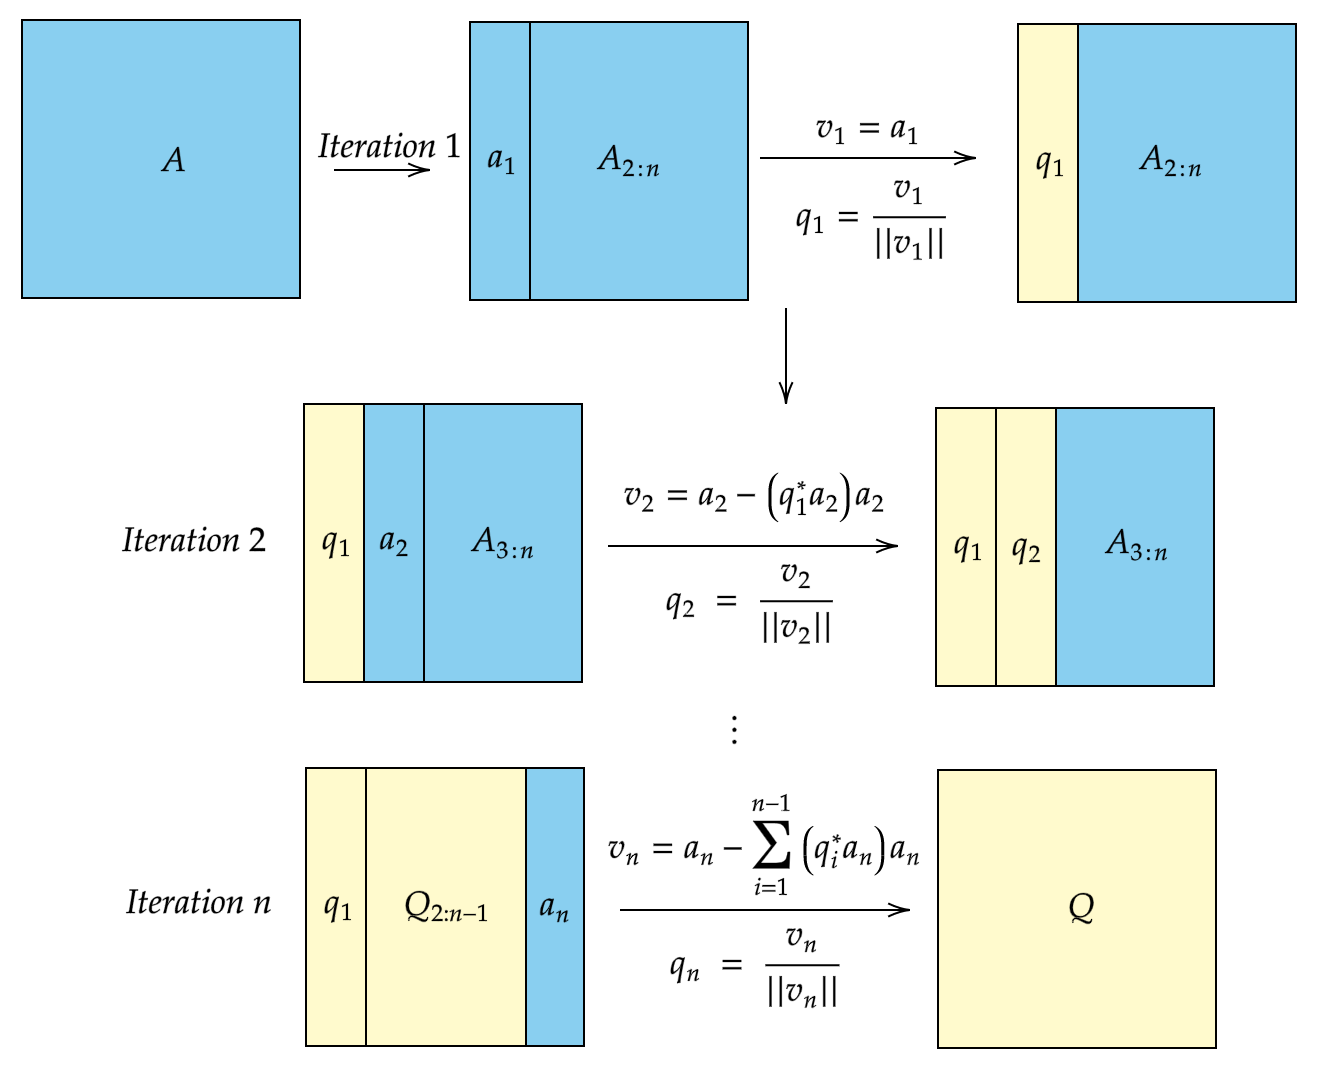
\includegraphics[width=\textwidth]{imgs/cgs.png}
  \caption{Classical Gram-Schmidt Algorithm Demonstration}
  \label{cgs}
\end{figure}

\noindent The only difference between the algorithm and \autoref{cgs} is I didn't create another array to store column-vectors of \(Q\) but in the sense of "converting" \(A\)  to \(Q\)  column-wise.
\newpage
\subsection*{Exercise 2.4: Implement the Classical Gram-Schmidt Algorithm}
\addcontentsline{toc}{subsection}{Exercise 2.4: Implement the Classical Gram-Schmidt Algorithm}
\subsubsection*{Problem Description}%
Here you need to implement the classical Gram-Schmidt algorithm from the derivation above in your function \href{https://comp-lin-alg.github.io/cla_utils.html#cla_utils.exercises2.GS_classical}{\texttt{exercises2.GS\_classical()}}. Note that instead returning matrices \(Q\) and \(R\) from the function, you need to change original matrix \(A\) to \(Q\) 'in-place' (which is in the way I demonstrated in \autoref{cgs}) and return \(R\) only.
\subsubsection*{What to do}
There is not too much to talk about in this exercise. However, two things are still worth mentioning:
\begin{enumerate}
  \item You are asked to change \(A\)  to \(Q\)  "in-place", which is not mentioned in the pseudo-code above. A good initiative to achieve this is to initialise \texttt{Q = A} in your function and follow the optimised algorithm to write your code. 
  \item When creating empty or zero matrices with NumPy, the matrices would not be initialised as complex matrices. You might find specifying \texttt{dtype=np.complex128} or \texttt{dtype=A.dtype} useful in your code implementation.  
\end{enumerate}
The main task for you now is to not be confused between indexes in maths formulas and Python (starting from 0). Try using 'vectorized' operations in your implementation, e.g. matrix multiplication rather than additional loops. \medskip

\noindent \textbf{Remember to check your implementation passes the provided test cases.}

\section{QR Factorisation by Modified Gram-Schmidt}
This part is the modification of classical Gram-Schmidt and contains two coding exercises. The initiative we want to make a modified version of classical Gram-Schmidt is due to the instability of classical GS. Here is the demonstration:\medskip

\noindent Let us say we have obtained \(Q, R\) from classical Gram-Schmidt, and mathematically we should have \(QR = A\). But since there are lots of rounding errors from the inexact arithmetic when this algorithm runs on computers, the entries of \(Q, R\)  are "polluted" so it is not necessarily correct for the equation \(QR = A\) when we do factorisation with classical GS. \medskip

\noindent Therefore the mathematicians propose a quick fix to the classical GS algorithm, and we called the modified version as \textbf{modified Gram-Schmidt}. The algorithm goes in this way:

\begin{algorithm}
\caption{Modified Gram-Schmidt Algorithm}
\label{mgs-algorithm}
\begin{algorithmic}[1]
\Procedure{GS\_modified}{A}
  \State initialise \(Q, R\)  as empty matrices
  \For{ \(i = 1\) to \(n\)}
    \State \(v_i = a_i\)
    \State \(r_{ii} = \frac{v_i}{\|v_i\|}\)  
    \For{ \(j = i + 1\) to \(n\)}
      \State \(r_{ij} = q_i^{*}v_j\)
      \State \(v_j = v_j - r_{ij}q_i\)
      \Comment{Remove components of \(q_i\) from all \(v_j\)s}
    \EndFor
    \Comment{Finish constructing a new basis vector \(q_j\)}
  \EndFor
  \State \Return \(Q, R\)
\EndProcedure
\end{algorithmic}
\end{algorithm}

\noindent To let you have a more direct sense of modified Gram-Schmidt, \autoref{mgs} would demonstrate the flow of the modified Gram-Schmidt Algorithm. \medskip
\begin{figure}[H]
  \centering
  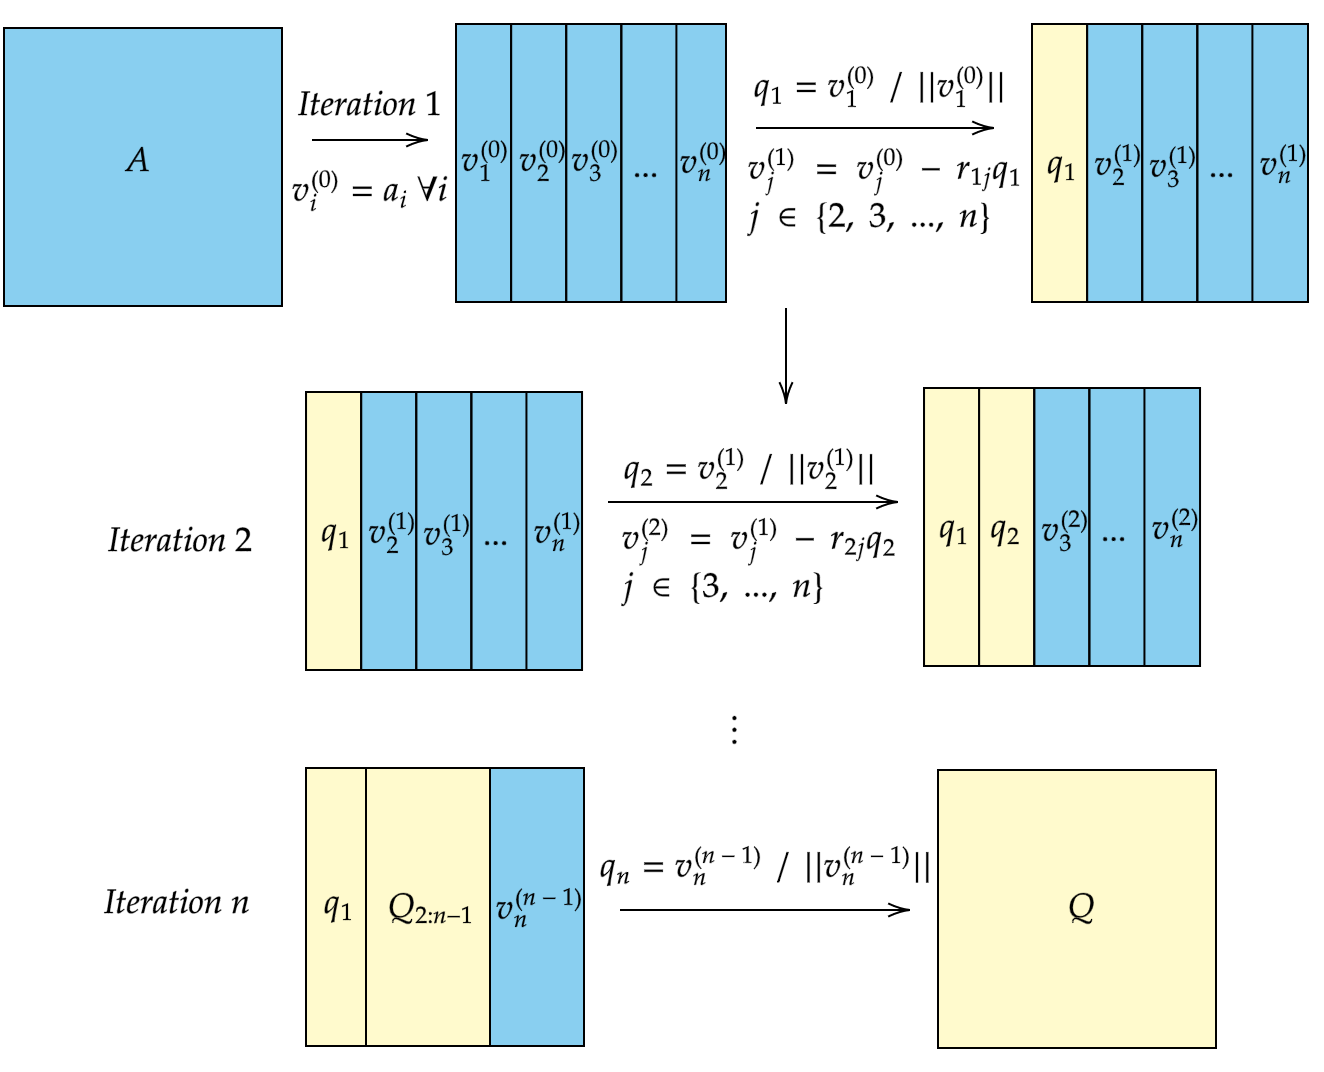
\includegraphics[width=0.9\textwidth]{imgs/mgs.png}
  \caption{Modified Gram-Schmidt Algorithm Demonstration}
  \label{mgs}
\end{figure}
\noindent You might find it confusing that, there are also superscripts in \(v_k\)  in \autoref{mgs} above, e.g. \(v_3^{(2)}\). The notation \(v_k^{(i)}\)  here is just for demonstrating the updated value of column vector \(v_k\) after iteration \(i\). 

\noindent For simplicity, I will ignore the superscripts \(^{(i)}\) in \(v_k\) in the following explanations, and I hope you could still understand the upcoming contents. \medskip

\noindent Essentially the modified GS and the classical GS have the same effect in factorisation. Recall that in classical GS what we did in each iteration \(k\) is, \textbf{set the vector \(v_k = a_k\), remove the components of found \(\{q_1, q_2, ..., q_{k - 1}\}\) from \(v_k\), set the normalised (and updated) \(v_k\) as \(q_k\), and add the obtained \(q_k\)  to the existing orthonormal set \(\{q_i\}\)} for the next iteration. However, what we did in the modified GS is, for each iteration \(k\), \textbf{I picked up the column vector \(v_k\), normalise it to obtain a basis vector \(q_k\), and remove the components of \(q_k\) from the vectors \(\{v_{k + 1}, ..., v_{n}\}\)} behind. \medskip

\noindent The two algorithms indeed have the same effect on an arbitrary matrix \(A\), and also have the same number of computational operations. However, the main difference is that in modified GS we define \(r_{ij} = q_i^{*}v_j\) rather than \(r_{ij} = q_i^{*}a_j\). In this case, \textbf{the rounding error} in finding \(r_{ij}\) would be \textbf{smaller} and the \textbf{algorithm will be more stable.} Click \href{https://math.stackexchange.com/questions/3913710/intuitive-explanation-of-why-the-modified-gram-schmidt-is-more-stable-than-the-c}{here} to see the explanation.\medskip

\noindent You might think now you should be ready for implementing this algorithm by yourself. However, from one of the gist in this course, \textbf{you should use avoid "additional" for loops as much as possible}. That is to say, you should consider if you could reduce the number of "for loops" in the algorithm shown in the class/on the website. Pause here for a while to think about it, and go to the next page for checking my solution to reduce no. of for-loops by introducing vectorized operations. 

\newpage
\noindent Consider the inner for-loop starting from \textbf{line 6 to line 9} in \autoref{mgs-algorithm}. Firstly we should see in this loop we computed the values \(\{r_{i(i + 1)}, r_{i(i + 2)}, ..., r_n\}\), by arithmetic we should see
\[
  r_i^{(i + 1, n)} = \begin{pmatrix} 
    r_{i(i + 1)} \\ r_{i(i + 2)} \\ \vdots \\ r_n
  \end{pmatrix}
  = 
  \begin{pmatrix} 
      q_i^{*}v_{i + 1} \\
      q_i^{*}v_{i + 2} \\
      \vdots \\
      q_i^{*}v_{n}
  \end{pmatrix}
  = \begin{pmatrix} 
     v_{i + 1}^{*}q_i & v_{i + 2}^{*}q_i & ... & v_{n}^{*}q_i
  \end{pmatrix}^{*}
\]
\[
  =
  (\begin{pmatrix} 
    v_{i + 1}^{*}q_i \\
    v_{i + 2}^{*}q_i \\
    \vdots \\
    v_{n}^{*}q_i
\end{pmatrix}^{\top})^{*}
  = ((V_{i + 1}^{*}q_i)^{\top})^{*} = ((V_{i + 1}^{*}q_i)^{*})^{\top} 
\]
\[
  = (q_i^{*}V_{i + 1})^{\top} = V_{i + 1}^{\top}\overline{q_i}
\]
where \(V_{i + 1} = \begin{pmatrix} 
    v_{i + 1} & v_{i + 2} & ... & v_{n}
\end{pmatrix} \)  and \(\overline{q_i}\) is the complex conjugate of \(q_i\). \medskip

\noindent Also we could see the component of \(q_i\)  is removed from \(\{v_{i + 1}, v_{i + 2}, ..., v_{n}\} \) in iteration \(i\). Recall the definition of outer product \(uv^{\top}\) and we should see
\[
  V_{i + 1} = V_{i + 1}
  - \begin{pmatrix} 
    r_{i(i + 1)}q_i & r_{i(i + 2)}q_i & ... & r_{in}q_i 
  \end{pmatrix} 
\]
\[
  = V_{i + 1} - q_i \begin{pmatrix} 
    r_{i(i + 1)} \\
    r_{i(i + 2)} \\
    \vdots \\
    r_{in}
  \end{pmatrix}^{\top}
  = V_{i + 1} - q_i (r_i^{(i + 1, n)})^{\top}
\]
Therefore, you now have the optimised version of the modified Gram-Schmidt algorithm, which is not mentioned by the lecturer but you would lose marks if not optimised.

\begin{algorithm}
  \caption{Modified Gram-Schmidt Algorithm, optimised}
  \label{mgs-algorithm-optimised}
  \begin{algorithmic}[1]
  \Procedure{GS\_modified\_optimised}{A}
    \State initialise \(Q, R\)  as empty matrices
    \For{ \(i = 1\) to \(n\)}
      \State \(v_i = a_i\)
      \State \(r_{ii} = \frac{v_i}{\|v_i\|}\)
      \State \(r_i^{(i + 1, n)} = V_{i + 1}^{\top}\overline{q_i}\)
      \State \(V_{i + 1} = V_{i + 1} - \overline{q_i} (r_i^{(i + 1, n)})^{\top}\)    
    \EndFor
    \State \Return \(Q, R\)
  \EndProcedure
  \end{algorithmic}
  \end{algorithm}

\subsection*{Exercise 2.5: Implement the Modified Gram-Schmidt Algorithm}
\addcontentsline{toc}{subsection}{Exercise 2.5: Implement the Modified Gram-Schmidt Algorithm}
\subsubsection*{Problem Description}%
You are now asked to implement the modified Gram-Schmidt algorithm in \href{https://comp-lin-alg.github.io/cla_utils.html#cla_utils.exercises2.GS_modified}{\texttt{exercises2.GS\_modified}}. You should be able to implement it with the minimum amount of loops from reading the optimised algorithm above. \medskip

\noindent \textbf{Remember to check your implementation passes the provided test cases.}

\section{Modified Gram-Schmidt Algorithm with Triangular Orthogonalisation}
From \autoref{mgs} you should see how modified Gram-Schmidt works iteratively. However, from another perspective, we could consider each iteration \(k\) as a transformation represented by matrix \(R_k\). Let us say $\hat{A}_0 = A$ and $\hat{A}_{k} = \hat{A}_{k - 1}R_k$, the transformation \(R_k\) should satisfy the following criteria:
\[
  \hat{A}_0 = \begin{pmatrix} v_{1}^{(0)} & v_{2}^{(0)} & \ldots & v_{n}^{(0)}\end{pmatrix} = A
\] and 
\[
  \hat{A}_{k} = \begin{pmatrix} v_1^{(k)} & v_2^{(k)} & \ldots & v_{n}^{(k)} \end{pmatrix} = \hat{A}_{k - 1}R_{k}
\] 
\begin{enumerate}
  \item The first $k - 1$ columns in $\hat{A}_{k - 1}$ and $\hat{A}_{k}$ should be the same after transformation. i.e. 
  \[
    \begin{pmatrix} v_1^{(k - 1)} & \ldots & v_{k - 1}^{(k - 1)} \end{pmatrix} = \begin{pmatrix} v_1^{(k)} & \ldots & v_{k - 1}^{(k)} \end{pmatrix} 
  \] 
  \item The $k$-th column in $\hat{A}_{k}$ is the normalised vector of column $k$ in $\hat{A}_{k - 1}$. i.e.
    \[
    v_{k}^{(k)} = \frac{v_{k}^{(k - 1)}}{\|v_{k}^{(k - 1)}\|}
    \] 
  \item The last $(n - k)$ columns in $\hat{A}_{k}$ is transformed from $\hat{A}_{k - 1}$ where
    \[
      v_{i}^{(k)} = v_{i}^{(k - 1)} - r_{ki} \frac{v_k^{(k - 1)}}{\|v_{k}^{(k - 1)}\|} = v_{i}^{(k - 1)} - \frac{r_{ki}}{r_{kk}}v_{k}^{(k - 1)} ~\forall i \in \{k + 1, k + 2, \ldots, n\} 
    \] 
    where
    \[
      r_{kk} = \|v_{k}^{(k - 1)}\|, r_{ki} = q_k^{*}v_{i}^{(k - 1)} = \frac{(v_k^{(k - 1)})^{*}v_{i}^{(k - 1)}}{\|v_{k}^{(k - 1)}\|}
    \]  
\end{enumerate}
Recall here we use the notation \(v_l^{(r)}\) for demonstrating the updated value of column vector \(v_l\) after iteration \(r\).
\begin{itemize}
  \item From the \textbf{Criteria 1} we could see that, when $1 \le  l \le  k - 1$, the $l$-th column vector of $\hat{R}_{k}$ should be the base vector $e_{l}$. i.e. the $r$-th element in vector $e_l$ is represented as the Kronecker delta $\delta_{lr}$.
  \item From the \textbf{Criteria 2} we could see that the $k$-th column vector of $ \hat{R}_{k}$ should be $\frac{e_k}{r_{kk}}$ in which $e_k$ follows the same definition as above.
  \item From the  \textbf{Criteria 3} we could see that the last $(n - k)$ columns of $\hat{R}_{k}$ (say the column $i$ is called $r_{k}^{(i)}$) should be in the form
    \[
      [r_{k}^{(i)}]_j = \left\{
        \begin{array}{ccl}
          1 &~ & $j = i$ \\
          -\frac{r_{ki}}{r_{kk}} & ~&$j = k$ \\
          0 & ~&\text{otherwise}
        \end{array}
      \right.
    .\] 
\end{itemize}
Therefore, the matrix $\hat{R}_{k}$ should take the form when $k = 2$:
\[
  \hat{R}_{k} = \begin{pmatrix}
  1 & 0 & 0 & \ldots & 0 \\
  0 & \frac{1}{r_{22}} & -\frac{r_{23}}{r_{22}} & \ldots & -\frac{r_{2n}}{r_{22}} \\
  0 & 0 & 1 & \ldots & 0 \\
  \vdots & \ddots & \ddots & \ddots & \vdots \\
  0 & \ldots & 0 & \ldots & 1
\end{pmatrix} 
\]
i.e. A $n \times n$ identity matrix except row $k$ is filled starting from the diagonal element $r_{kk}$, where the diagonal element is $\frac{1}{r_{kk}}$ and the elements behind the element takes the form $-\frac{r_{ki}}{r_{kk}}$, where $i$ is the column index. In which case
\[
  \{-\frac{r_{ki}}{r_{kk}}\} = \begin{pmatrix} 
    - \frac{r_{k(k + 1)}}{r_{kk}} \\ -\frac{r_{k(k + 1)}}{r_{kk}} \\ \vdots \\ -\frac{r_{kn}}{r_{kk}}
  \end{pmatrix} = -\frac{1}{\|v_{k}^{(k - 1)}\|}\begin{pmatrix} 
    (v_k^{(k - 1)})^{*}v_{k + 1}^{(k - 1)} \\
    (v_k^{(k - 1)})^{*}v_{k + 2}^{(k - 1)} \\
    \vdots \\
    (v_k^{(k - 1)})^{*}v_{n}^{(k - 1)}
  \end{pmatrix} = -\frac{(V_{k + 1}^{(k - 1)})^{\top}\overline{v_k^{(k - 1)}}}{\|v_{k}^{(k - 1)}\|}
\]
where \(V_{k + 1}^{(k - 1)} = \begin{pmatrix} 
  v_{k + 1}^{(k - 1)} & v_{k + 2}^{(k - 1)} & ... & v_{n}^{(k - 1)}
\end{pmatrix} \). i.e. the last \(n - k\) cols of \(\hat{A}_{k - 1}\).  \medskip

\noindent You should also see that inductively the $\hat{Q}$ obtained from this method takes this form:
\[
\hat{Q} = A \hat{R}_1 \hat{R}_2 \ldots \hat{R}_n
\] 
And since every $\hat{R}_k$ is essentially an upper triangular matrix, so do their products. We know that the inverse of an upper triangular matrix is still upper triangular, so we could obtain $\hat{R}$ from the inverse of product $\prod_{k=1}^{n}\hat{R}_k$. \medskip

\noindent Also here we are using a series of \textbf{upper triangular} matrices to obtain an orthogonal matrix $\hat{Q}$, and this is the reason we called it \textbf{triangular orthogonalisation}. The algorithm with triangular orthogonalisation in modified Gram-Schmidt is shown below:

\begin{algorithm}[H]
  \caption{Get \(R_k\) for triangular orthogonalisation in modified GS}
  \label{mgs-get-r}
  \begin{algorithmic}[1]
  \Procedure{GS\_modified\_get\_R}{$\hat{A}_{k - 1}$, $k$} 
    \State initialise \(\hat{R}_k\)  as an identity matrix
    \State \(\hat{R}_{k}\)\texttt{[k, k]} \(= \|\hat{A}_{k - 1}\texttt{[:, k]}\|\)
    \State \(\hat{R}_{k}\)\texttt{[k, k + 1:]} \(=- \frac{\hat{A}_{k - 1}\texttt{[:, k + 1:]}^{\top} \overline{\hat{A}_{k - 1}\texttt{[:, k]}}}{\hat{R}_{k}\texttt{[k, k]}}\)       
    \State \Return \(\hat{R}_k\)
  \EndProcedure
  \end{algorithmic}
  \end{algorithm}
\noindent Note that some implementations of this algorithm will not explicitly mention \(\hat{A}_{k - 1}\) as the input parameter, instead the input parameter would be a general matrix \(A\). Keep this in mind and you might need this in exercise. 
\begin{algorithm}[H]
  \caption{Modified Gram-Schmidt with Triangular Orthogonalisation}
  \label{mgs-r}
  \begin{algorithmic}[1]
  \Procedure{GS\_modified\_R}{$A$} 
    \State \texttt{m, n = A.shape}
    \State initialise \(Q, R\) as \(A\) and an identity matrix
    \For{ \(k = 1\) to \(n\)}
      \State \(\hat{R}_k = \)  GS\_MODIFIED\_GET\_R\((A, k)\)
      \State \(Q = Q \hat{R}_{k}\)
      \State \(R = R \hat{R}_{k}\)     
    \EndFor
    \State \Return \(Q, R\)
  \EndProcedure
  \end{algorithmic}
  \end{algorithm}

  \subsection*{Exercise 2.6: Implement the \texttt{get\_R()} Function Modified GS}
  \addcontentsline{toc}{subsection}{Exercise 2.6: Implement the \texttt{get\_R()} Function Modified GS}
  \subsubsection*{Problem Description}%
  You are now asked to implement the modified Gram-Schmidt algorithm in \href{https://comp-lin-alg.github.io/cla_utils.html#cla_utils.exercises2.GS_modified_get_R}{\texttt{exercises2.GS\_modified\_get\_R}}. You should be able to implement it with reference of \autoref{mgs-get-r}. \medskip
  
\noindent \textbf{Remember to check your implementation passes the provided test cases.}


 \bigskip

 \begin{center}
   \textit{\large End of Week 2}
 \end{center}
